\documentclass[12pt,a4paper]{article}

\usepackage{fullpage}
\usepackage{parskip}
\usepackage{amsmath}
\usepackage{amssymb}
\usepackage{hyperref}
\usepackage{bm}
\usepackage{enumerate}
\usepackage{enumitem}
\usepackage{graphicx}
\usepackage{booktabs}

\newcommand{\pluseq}{\mathrel{+}=}
\newcommand{\asteq}{\mathrel{*}=}
\newcommand{\norm}[1]{\left\lVert#1\right\rVert}

\title{Pattern Recognition Assignment 3: K-Means}
\author{Yu Hao\\[10pt] Student ID: 1831607}

\date{\today}

\begin{document}

\maketitle

\section{Introduction}
In this assignment, we are expected to implement a clustering algorithm. There are many kinds of methods for clustering, for example, K-Means, hierarchical clustering, DBSCAN, etc. I choose standard K-Means as the basic method and there will be some extensions to be mentioned later. As we confront a real problem from Huawei project which needs to partition dataset equally under the condition of minimizing within-cluster sum of squares (WCSS), we propose an extension of K-means to accomplish the objective.

Hence, the assignment is organized by two parts: the standard K-Means implementation and its extension. Furthermore, the second part will be filled and plump at our team's final project.
\section{Algorithm Formulation}
Given a set of data points $\mathbf{H}=\left \{ \bm{h}_{1},\ldots,\bm{h}_{N} \right \}$, where each point is a d-dimensional real-valued vector.
The aim of K-means algorithm is to divide $N$ data points into $K\ (\leqslant N)$ sets $\mathbf{C}=\left \{ \mathit{C}_{1},\ldots,\mathit{C}_{K} \right \}$
so as to minimize the within-cluster sum of squares (WCSS) function. Formally, the objective is to find
\begin{equation}
\begin{aligned}
\underset{\mathbf{C}}{\rm argmin}~&\sum\nolimits_{k=1}^{K}\sum\nolimits_{i\in C_{k}} \norm{ \bm{h}_{i}-\bm{c}_{k}}^{2}\\[6pt]
&=\sum\nolimits_i{ \norm{\bm{h}_i}^{2}} -\sum\nolimits_{k=1}^{K}\frac{1}{n_k}\sum\nolimits_{i,j\in C_{k}}{\bm{h}_{i}}^{T}\bm{h}_{j},
\end{aligned}
\end{equation}
where $\bm{c}_{k}$ represents the centroid of cluster $C_{k}$ for $k=1,2,\ldots,K$ and $\bm{n}={[n_{1},\ldots,n_{K}]}^{T}\in \mathbb{R}^{K}$ records the number of data points for $K$ clusters.
The optimization process is known as a NP-hard problem~\cite{garey1982complexity}, and the standard K-means algorithm  \cite{hartigan1975clustering} was proposed to provide an approximate solution. The algorithm uses an iterative refinement technique. Given an initial set of $K$ centroids $\{ \bm{c}_{1}^{(0)},\bm{c}_{2}^{(0)},\ldots,\bm{c}_{K}^{(0)}\}$, the algorithm proceeds with alternating strategy between an assignment step and an update step as follows.

During the assignment step, each data point is assigned to the cluster characterized by nearest centroid, that is
\begin{equation}
\begin{aligned}
C_{k}^{\left(t\right)}&=\left \{{ \mathbf {h}_{p}:\left \|{\mathbf {h}_{p} - \mathbf {c}_{k}^{\left(t\right)}}\right \|^{2}\le \left \|{ \mathbf {h}_{p} - \mathbf {c}_{j}^{\left(t\right)} }\right \|^{2}, 1\leq j\leq K }\right \}, \\[6pt]
n_{k}^{\left(t\right)}&=|C_{k}^{\left(t\right)}|, \\[6pt]
k&=1,\ldots , K,
\end{aligned}
\end{equation}
where each data point is assigned to exactly one cluster, and this step can minimize the WCSS function.

During the update step, the new centroids can be computed with current clusters:
\begin{equation} 
\mathbf c_{k} ^{\left ({t+1}\right )} = \frac {1}{n_{k}^{(t)}} \sum _{\mathbf h_{j} \in C_{k}^{\left ({t}\right )}} \mathbf h_{j},~k=1,\ldots ,K. 
\end{equation}
Since the arithmetic mean is a least-squares estimator, this step also minimizes the WCSS function.

The algorithm converges when the centroids no longer change, in other words, the data points are no longer assigned to new cluster. The K-means algorithm can converge to a local optimum. Since for a given $K$, the result of above clustering algorithm depends solely on the initial centroids.

The computational complexity of the K-means algorithm is $O(NdKM)$, where $N$ is the number of the d-dimensional vectors, $K$ is the number of clusters and $M$ is the number of iterations before reaching convergence.

\section{K-Means Implementation}
Three parts will be mentioned there. Similar with former assignments, I choose two datasets: The mobile prices classifications and glasses types classifications. Algorithm implementation consists of three parts, which are centroids initialization, update data points assignments, and recalculate centroids. After acquiring the result, we will compare clustering results with true labels to examine the clustering quality. Visualization is the last implementation to see the result clearly.

\subsection{Data Preprocessing}
We have two datasets and both of them are numerical, so I just need to normalize the features. The purpose of normalization is to avoid the influences of features' order of magnitudes, rather focus on their distributions and relative distances. Standardizing is very simple:
\begin{equation}
z=\frac{x-\mu}{\sigma},
\end{equation}
where $x$ is the number to be standardized, $\mu$ is the feature's mean, and $\sigma$ is the standard deviation. 

\subsection{Fit}
This module is to do the clustering. Firstly we need to choose $K$ centroids as the initial centroids. I choose the corresponding data points from the dataset as the centroids. There are some input checks. The algorithm cannot handle the circumstance that the number of clusters bigger than data points'. And obviously, the clusters number needs to be a positive integer.

Then we iterate the next two steps until the \textbf{centroids} don't change anymore:
\begin{itemize}
	\item Update assignments. I calculate the Euclidean distances from all data points to all centroids and choose the closest centroid to be the representative of each point. After accomplishing the calculation, I record the result to an array: \textbf{clustering\_results}.

	\item Recalculate centroids. For the data points belong to the same cluster, they need a new representative. For simplicity, the mean of these data points is a suitable choice. I denote the result as \textbf{centroids}.
\end{itemize}

\subsection{Result Comparison}
As the dataset has true labels, we can examine the quality of clustering using Adjusted Rand index. The Rand index in data clustering is a measure for calculating the similarity between two data clusterings. From a mathematical standpoint, the Rand index is related to the accuracy but is applicable even when class labels are not used.
\subsubsection{Rand index}
Given a set of $N$ elements $\mathbf{S}=\left\{s_1,\ldots,s_N\right\}$ and two partitions of $\mathbf{S}$ to compare, $\mathbf{X}=\left\{X_1,\ldots,X_K\right\}$, a partition of $\mathbf{S}$ into $K$ subsets, and $\mathbf{Y}=\left\{Y_1,\ldots,Y_Q\right\}$, a partition of $\mathbf{S}$ into $Q$ subsets. define the following:
\begin{itemize}
	\item $a$, the number of pairs of elements in $\mathbf{S}$ that are in the same subset in $\mathbf{X}$ and in the same subset in $\mathbf{Y}$;
	\item $b$, the number of pairs of elements in $\mathbf{S}$ that are in different subsets in $\mathbf{X}$ and in different subsets in $\mathbf{Y}$;
	\item $c$, the number of pairs of elements in $\mathbf{S}$ that are in the same subset in $\mathbf{X}$ and in different subsets in $\mathbf{Y}$;
	\item $b$, the number of pairs of elements in $\mathbf{S}$ that are in different subsets in $\mathbf{X}$ and in the same subset in $\mathbf{Y}$.
\end{itemize}
The Rand index, $R$, is:
\begin{equation}
R=\frac{a+b}{a+b+c+d}=\frac{a+b}{\binom{N}{2}}.
\end{equation}

Intuitively, $a+b$ can be considered as the number of agreements between $\mathbf{X}$ and $\mathbf{Y}$, and $c+d$ as the number of disagreement between them. Since the denominator is the total number of pairs, the Rand index represents the frequency of occurrence of agreement over the total pairs or the probability that $\mathbf{X}$ and $\mathbf{Y}$ will agree on a randomly chosen pair.

\subsubsection{Adjusted Rand index}
The adjusted Rand index is the corrected-for-chance version of the Rand index. Such a correction for chance establishes a baseline by using the expected similarity of all pair-wise comparisons between clusterings specified by a random model. Traditionally, the Rand Index was corrected using the Permutation Model for clusterings (the number and size of clusters within a clustering are fixed, and all random clusterings are generated by shuffling the elements between the fixed clusters). However, the premises of the permutation model are frequently violated; in many clustering scenarios, either the number of clusters or the size distribution of those clusters vary drastically. For example, consider that in K-Means the number of clusters is fixed by the practitioner, but the sizes of those clusters are inferred from the data. Variations of the adjusted Rand Index account for different models of random clusterings.

Though the Rand Index may only yield a value between 0 and +1, the adjusted Rand index can yield negative values if the index is less than the expected index.

Given a set S of $N$ elements, and two groupings or partitions (e.g. clusterings) of these elements, namely $\mathbf{X}=\{X_{1},X_{2},\ldots ,X_{K}\}$ and $\mathbf{Y}=\{Y_{1},Y_{2},\ldots ,Y_{Q}\}$, the overlap between X and Y can be summarized in a contingency table $\left[n_{ij}\right]$ where each entry $n_{ij}$ denotes the number of objects in common between $X_i$ and $Y_j$: $n_{ij}=|X_{i} \cap Y_{j}|$.

\begin{table}
\centering
\begin{tabular}{c c c c c c}
\hline
\hline
~ & $Y_1$ &	$Y_2$ &	$\cdots$ & $Y_Q$  & Sums \\[6pt]
\hline
$X_1$ &	$n_{11}$ & 	$n_{12}$ & 	$\cdots$  &	$n_{1Q}$  &	$a_1$ \\[6pt]
\hline
$X_2$ & $n_{21}$ 	& $n_{22} $	& $\cdots$	& $n_{2Q}$	& $a_2$ \\[6pt]
\hline
$\vdots$ & $\vdots$ & $\vdots$ & $\ddots$ & $\vdots$ & $\vdots$ \\[6pt]
\hline
$X_K$ & $n_{K1}$ & $n_{K2}$ & $\cdots$ & $n_{KQ}$ & $a_K$ \\[6pt]
\hline
$Sums$ & $b_1$ & $b_2$ & $\cdots$ &$b_Q$ & ~\\[6pt]
\hline
\hline
\end{tabular}
\caption{contingency table}
\end{table}

The original Adjusted Rand Index using the Permutation Model is
\begin{equation}
\begin{aligned}
ARI &= \frac{Index-ExpectedIndex}{MaxIndex-ExpectedIndex} \\[6pt]
Index &= \sum_{ij}\binom{n_{ij}}{2} \\[6pt]
ExpectedIndex &= \frac{\sum_{i}\binom{a_i}{2}\sum_{j}\binom{b_j}{2}}{\binom{N}{2}} \\[6pt]
MaxIndex &= \frac{\sum_{i}\binom{a_i}{2}+\sum_{j}\binom{b_j}{2}}{2}
\end{aligned}
\end{equation}

Hence, the $ARI$ can be an effective index to examine the similarity between the clustering result and true classification. For the two datasets I mentioned, table \ref{ARI result} shows simulation result.

\begin{table}
\centering
\begin{tabular}{l l l l}
\hline
\hline
Dataset & Number of dataset & Number of clusters & ARI \\[6pt]
\hline
mobile prices classes & 2000 & 4 & 0.466 \\[6pt]
\hline
glasses types & 142 & 7 & 0.598 \\[6pt]
\hline
\hline
\end{tabular}
\caption{ARI of two datasets \label{ARI result}}
\end{table}

\subsection{Visualization}
Here I draw the true classifications and clustering (predicting) results in pictures using different colors to classify corresponding clusters.

\begin{figure}
\centering
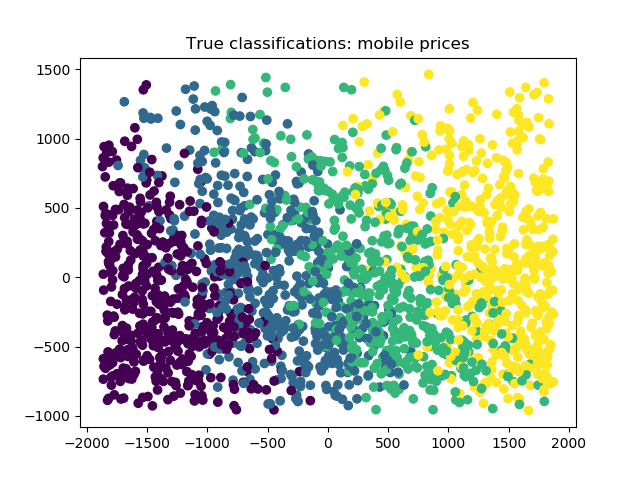
\includegraphics[width=11cm]{mobile-true}
\caption{Mobile prices classes: True result}
\label{mobile-true}
\end{figure}

\begin{figure}
\centering
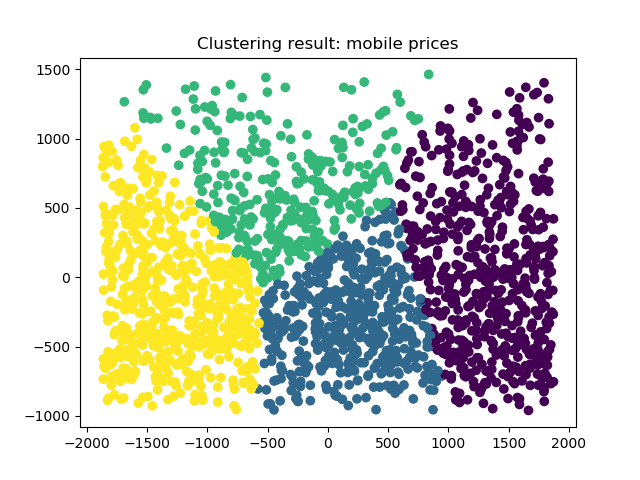
\includegraphics[width=11cm]{mobile-predict}
\caption{Mobile prices classes: Predicting result}
\label{mobile-predict}
\end{figure}

\begin{figure}
\centering
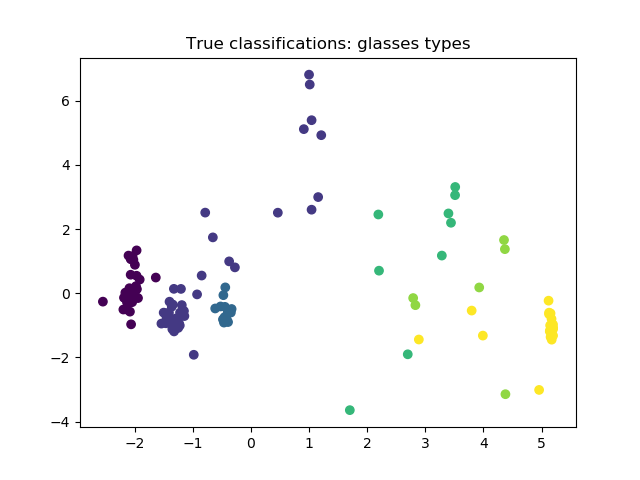
\includegraphics[width=11cm]{glasses-true}
\caption{Glasses types: True result}
\label{glasses-true}
\end{figure}

\begin{figure}
\centering
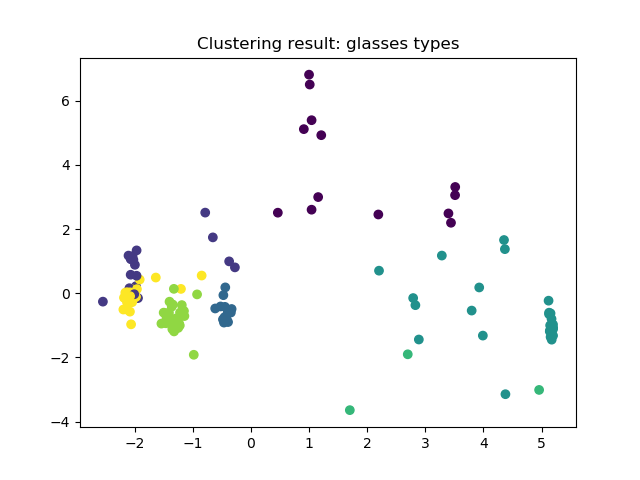
\includegraphics[width=11cm]{glasses-predict}
\caption{Glasses types: Predicting result}
\label{glasses-predict}
\end{figure}

Compare figure \ref{mobile-true} and \ref{mobile-predict}, we can see that the true result is a parallel-shaped figure with overlaps whereas K-Means cannot partition like that. In fact, I think it's a challenge for most clustering methods. For the sparser dataset, glasses, it has some obvious centers in distribution. Intuitively, it is easier to be partitioned, and the $ARI$ proves the assumption.

\section{Improvement of K-Means}
K-Means has been proposed for many years and it has a lot of perfection versions now. We just list some representative works here.

\subsection{Advantages and Disadvantages of K-Means}
\subsubsection{Advantages}
\begin{itemize}
\item Easy to implement.
\item With a large number of variables, K-Means may be computationally faster than hierarchical clustering (if $K$ is small). 
\item k-Means may produce tighter clusters than hierarchical clustering.
\item An instance can change cluster (move to another cluster) when the centroids are recomputed.
\end{itemize}
\subsubsection{Disadvantages}
\begin{itemize}
\item Difficult to predict the number of clusters (K-Value).
\item Initial seeds have a strong impact on the final results.
\item The order of the data has an impact on the final results.
\item Sensitive to scale: rescaling your datasets (normalization or standardization) will completely change results. While this itself is not bad, not realizing that you have to spend extra attention (on to scaling your data might be bad).
\end{itemize}

\subsection{Variations of the K-Means Algorithm}
The K-Means algorithm can be classified into center-based clustering algorithms. These clustering algorithms were developed to improve the performance of the standard K-Means algorithm\cite{gan2007data}. We will address some of these algorithms in subsequent sections.
\subsubsection{The Continuous K-Means Algorithm}
The continuous K-Means algorithm, proposed by Faber, is faster than the standard K-Means algorithm. It is different from the standard K-Means algorithm in the following aspects. Firstly, in the continuous K-Means algorithm, the prototypes (or reference points) are chosen as a random sample from the whole database, while in the standard K-Means algorithm the initial points are chosen arbitrarily. Secondly, the data points are treated differently. During each complete iteration, the continuous K-Means algorithm examines only a sample of the data points, while the standard K-Means algorithm examines all the data points in sequence.

\subsubsection{The Compare-means Algorithm}
In order to accelerate the K-Means algorithm, the algorithm compare-means uses a simple approach to avoid many unnecessary comparisons. Since the number of clusters $K$ is usually small, distances of all pairs of means are precomputed before each iteration. Then, before comparing a point x to a mean $\mu_j$ , the above test is performed using the closest known mean to x.

\subsubsection{The Sort-means Algorithm}
The algorithm sort-means is an extension of compare-means. In this algorithm, the means are sorted in order of increasing distance from each mean in order to obtain a further speedup.

\subsubsection{Acceleration of the K-Means Algorithm with the kd-tree}
Pelleg and Moore proposed an algorithm for the K-Means clustering problem using the $kd$-tree data structure. The $kd$-tree data structure, can be used to reduce the large number of nearest-neighbor queries issued by the traditional K-Means algorithm. Hence, an analysis of the geometry of the current cluster centers can lead to a great reduction in the work needed to update the cluster centers. In addition, the initial centers of the K-Means algorithm can be chosen by the $kd$-tree efficiently. One way to use the $kd$-tree in the inner loop of the K-Means algorithm is to store the centers in the tree; another way is to store the whole data set in the tree. To describe the application of the $kd$-tree in the K-Means algorithm, let us start with an iteration of the K-Means algorithm. Let $C^{\left(i\right)}$ denote the set of centroids after the $i-th$ iteration. Before the first iteration,
$C^{\left(0\right)}$ is initialized to a set of random values. The stop criterion of the algorithm is that $C^{\left(i\right)}$ and $C^{\left(i-1\right)}$ are identical. In each iteration of the algorithm, the following two steps are performed:
\begin{enumerate}
\item For each data point $x$, find the center in $C^{\left(i\right)}$ that is closest to $x$ and associate $x$ with this center.
\item Update $C^{\left(i\right)}$ to $C^{\left(i+1\right)}$ by taking, for each center, the center of mass of all the data points associated with this center.
\end{enumerate}

\subsection{Our project's requirement}
The variations for K-Means above are mostly performing in the speed or the quality. We consider that K-Means cannot obtain the results with some constraints, like sizes. However, we need to partition our project's large-scale dataset into some uniform clusters so that we could solve the subproblems with similar scales concurrently. We cannot partition our original dataset directly as the elements in the set are relational. Hence, we have to adjust current methods to meet our requirement. K-Means has good expandability, which can be our foundation.

\section{Looking Forward: Clustering with Size Constraints}
This section will be our team's final project and the outline is disclosed in this assignment. Look forward to the main body at the final report and presentation.

\begin{itemize}
\item Matrix form of K-Means
\item Constraints description
\item Problem derivation
\item Problem optimization
\item Parallel solving
\item Simulation and comparison
\item Perfection under large-scale data
\end{itemize}

\clearpage

\bibliographystyle{IEEEtran}
\bibliography{ref}

\end{document}